\documentclass[12pt]{article}
\usepackage{graphicx} % Required for inserting images
\graphicspath{{images/}}
\usepackage{amsmath}
\usepackage[italian]{babel}
\usepackage{listings}
\usepackage{biblatex}
\addbibresource{libro-algoritmi.bib}

\title{Laboratorio di Algoritmi e Strutture dati Esercizio 1}
\author{Leonardo Guglielmi}
\date{September 2023}

\begin{document}
\maketitle
\tableofcontents
------------------------------------------------------------------------------------------------
% ==============================================================================================
% INTRODUZIONE GENERALE
% ==============================================================================================
\section{Introduzione generale}

\subsection{Obiettivo}
L'obiettivo di questo esperimento è quello di confrontare varie implementazioni delle strutture dati per rappresentare gli insiemi disgiunti.\\
Più precisamente si vogliono confrontare le implementazioni tramite liste concatenate, sia con che senza euristica dell'unione pesata, e tramite foreste di insiemi disgiunti con compressione del cammino.\\
Queste diverse implementazioni verranno confrontate basandosi sull'efficienza nell'eseguire algoritmi per il calcolo delle componenti connesse nei grafi non diretti.

\subsection{Una breve descrizione della relazione}
La relazione è suddivisa in 5 parti:
\begin{itemize}
    \item \textbf{Descrizione teorica:} si vanno a descrivere tutti gli aspetti teorici che interessano l'esperimento svolto.

    \item \textbf{Prestazioni attese:} si delineano le prestazioni attese delle varie parti dell'esperimento.

    \item \textbf{Descrizione degli esperimenti:} si va a descrivere in che modo gli esperimenti vengono svolti ed il codice che li esegue.

    \item \textbf{Risultati sperimentali:} si espongono i risultati ottenuti dall'esecuzione dell'esperimento, sia in modo descrittivo che graficamente.

    \item \textbf{Deduzioni finali:} una volta osservati i risultati, si vanno a dare le considerazioni finali su quanto i risultati coincidano con le ipotesi fatte.
\end{itemize}

\subsection{Specifiche tecniche}
A seguire si elencano tutte le caratteristiche della macchina su cui verrà eseguito l'esperimento:
\begin{itemize}
    \item modello: Asus vivobook S15
    \item sistema operativo: fedora (linux)
    \item processore: Intel Core i7-8565U 1.80 GHz
    \item RAM: 8 GB DDR-4
    \item disco: ssd Kingstone A2000 256 GB

\end{itemize}
Inoltre il linguaggio usato sarà Python 3.11.5, mentre il codice è stato scritto e testato usando l'IDE Pycharm Professional 2023.2.1
\\ Questa relazione è stata scritta usando l'editor online Overleaf.\\
Per la stesura di questa relazione e per la realizzazione di questo esperimento è stato preso come riferimento il libro \cite{2010Iaae} \textit{Introduzione agli algoritmi e strutture dati} di Thomas Cormen.


% ==============================================================================================
% DESCRIZIONE TEORICA
% ==============================================================================================
\section{Descrizione teorica}
\subsection{Strutture dati per insiemi disgiunti}
Le strutture dati per insiemi disgiunti, dette anche strutture Union-Find, sono utilizzate per rappresentare un insieme di collezioni disgiunte di elementi distinti, ognuna delle quali avrà uno dei suoi elementi come rappresentante.
\\Su queste strutture vengono svolte le generiche operazioni di:
\begin{itemize}
    \item \textit{make\_set(e)}: crea un nuovo insieme $\{e\}$ contente il solo elemento \textit{e}, il quale sarà rappresentante del nuovo inseme.
    \item \textit{union(A,B)}: unisce gli insiemi \textit{A} e \textit{B}, il nuovo insieme avrà come rappresentante il rappresentante di \textit{A}.
    \item \textit{find(e)}: restituisce il rappresentante dell'insieme in cui è contenuto \textit{e}.
\end{itemize}

\subsection{Rappresentazioni per gli insiemi disgiunti}
Benché il costo dell'operazione di \textit{make\_set} risulti sempre $O(1)$, il costo delle altre operazioni varia il base alle varie rappresentazioni, in particolare in questo esperimento verranno usate le seguenti:

    \subsubsection{Lista concatenata} In questa rappresentazione, detta anche \textit{QuickFind}, ciascun insieme è rappresentato da una lista concatenata.\\
    Ogni lista ha un puntatore \textit{head} che punta al primo elemento, il quale è anche rappresentante dell'insieme, ed un puntatore \textit{tail} che invece punta all'ultimo elemento della lista.\\
    Ciascun elemento della lista invece contiene l'identificativo dell'elemento dell'insieme, un puntatore all'oggetto lista ed un puntatore al successivo elemento.\\
    Tramite questa rappresentazione l'operazione di \textit{find} ha un'implementazione molto efficiente, in quanto deve soltanto seguire i puntatori.\\
    Per quanto riguarda l'operazione di \textit{union} questo tipo di rappresentazione risulta meno efficiente, essa infatti si realizza andando ad accodare una lista all'altra, dovendo quindi andare ad aggiornare il puntatore all'oggetto lista di tutti gli elementi appartenenti alla lista accodata, impiegando quindi un tempo al più lineare $\theta(n)$.

    \subsubsection{Foresta di insiemi disgiunti}  Con questa rappresentazione, detta anche \textit{QuickUnion}, ogni insieme è rappresentato da un albero.\\
    La radice dell'albero sarà il rappresentante dell'insieme e ogni elemento dell'insieme è rappresentato da un nodo, il quale contiene l'identificativo dell'elemento ed un puntatore al nodo padre \textit{father}.\\
    Nella radice il puntatore \textit{father} punterà a se stessa.\\
    Tramite tale rappresentazione si ha che l'implementazione dell'operazione di \textit{union} risulta molto semplice, in quanto si andrà a rendere uno dei due insiemi un sotto-albero della radice dell'altro: per implementare ciò si va a modificare il puntore \textit{father} della radice dell'insieme che vogliamo accodare, facendolo puntare alla radice dell'altro insieme.\\
    Tuttavia l'implementazione di \textit{find} risulta più problematica poiché si deve risalire dal nodo di partenza tutto l'albero fino alla radice tramite i puntatori \textit{father}, risultando più costosa rispetto a \textit{find} e \textit{make\_set}.\\
    Il cammino che si forma durante la ricerca viene detto \emph{cammino di ricerca}.

\subsection{Euristiche}
Esistono delle euristiche che permettono di migliorare i tempi di esecuzione delle operazioni più costose di ciascuna rappresentazione e delle relative implementazioni:

    \subsubsection{Euristica dell'unione pesata} usata nella rappresentazione tramite \textbf{lista concatenata}, quando si va a fare una \textit{union} si sceglie di accodare la lista con il minor numero di elementi a quella contenente più elementi, in modo da ridurre il numero di elementi da aggiornare.\\
    Questo richiede che la lista memorizzi anche il numero di elementi al suo interno.

    \subsubsection{Compressione del cammino} usata della rappresentazione tramite \textbf{foresta di insiemi disgiunti}, consiste nel rendere ogni nodo nel cammino di ricerca di una \textit{find} figlio della radice, andando quindi ad aggiornare il puntatore \textit{father} del nodo nel cammino in modo che punti direttamente alla radice.\\

    \subsection{Algoritmo per il calcolo delle componenti connesse}
    Infine, per costruire le \textbf{componenti connesse} verrà usato l'algoritmo per grafi non orientati (Figura \ref{fig:cc_pseudocode}), il quale eseguendo una serie di operazioni di \textit{make\_set, find} e \textit{union} andrà a creare una collezione di insiemi, ognuno rappresentante una componente connessa.\\
    \begin{figure}[h]
        \centering
        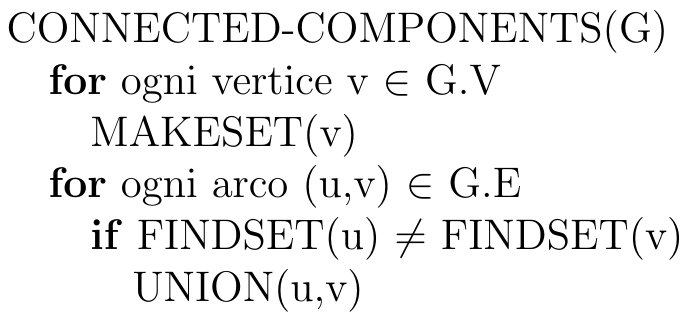
\includegraphics[width=0.5\textwidth]{images/cc_pseudocode.png }
        \caption{Pseudocodice algoritmo per il calcolo delle componenti connesse}
        \label{fig:cc_pseudocode}
    \end{figure}

\noindent L'esecuzione dell'algoritmo per il calcolo delle componenti connesse ha dei tempi di esecuzione molto differenti in base alla rappresentazione ed alle implementazioni usate:
    \begin{itemize}
        \item \textbf{Rappresentazione tramite liste concatenate:} creando $n$ insiemi con \textit{make\_set} impiego un tempo $\theta(n)$, se eseguo la union andando ad accodare la lista contente il maggior numero di elementi ho un tempo medio per chiamata dell'operazione di \textit{union} di $\theta(n)$, perciò in totale per una certa sequenza delle operazioni per gli insiemi disgiunti impiego un tempo $\theta(n^2)$.

        \item \textbf{Rappresentazione tramite liste concatenate con euristica pesata del cammino:} si ha che una sequenza di operazioni \emph{make\_set}, \emph{union} e \emph{find} impiega un tempo $O(m+n\cdot lg\ n)$, dove $n$ è il numero di operazioni di \emph{make\_set} e $m$ è il numero totale di operazioni eseguite.

        \item \textbf{Rappresentazione tramite foresta di insiemi disgiunti con compressione del cammino:} si ha che una sequenza di $m$ operazioni di \textit{make\_set},\textit{union} e \textit{find} richiedono un tempo $\theta(n + f\cdot (1 + log_{2+f/n}\ n))$, dove $n$ è il numero di operazioni \textit{make\_set} e $f$ il numero di \textit{find}.

    \end{itemize}

\section{Prestazione attese}
Ci si aspetta dunque che la rappresentazione tramite \textit{lista concatenata} risulti quella meno efficiente nell'eseguire l'algoritmo per il calcolo delle componenti connesse a causa del suo costo quadratico, mentre per le implementazioni tramite \textit{lista concatenata con euristica dell'unione pesata} e \textit{foresta di insiemi disgiunti} il tempo di esecuzione dipenderà dal numero di operazioni eseguite, per tale motivo si dovrà osservare come il numero di operazioni cresce alla dimensione del problema per avere un'idea di come il costo di queste due rappresentazioni cresca.

% ==============================================================================================
% DESCRIZIONE ESPERIMENTI E CODICE
% ==============================================================================================
\section{Descrizione esperimenti e codice}

Il codice è stato diviso in 3 moduli Python:
\begin{itemize}
    \item \textbf{linked\_list.py} contiene tutte le classi e le funzioni relative alla rappresentazione mediante lista concatenata, sia con che senza euristica dell'unione pesata.
    \item \textbf{set\_forest.py} contiene classi e funzioni relative alla rappresentazione mediante foresta di alberi disgiunti.
    \item \textbf{main.py} contiene il codice che inizializza le variabili dell'esperimento, esegue le simulazioni e riporta i risultati dell'esperimento.
\end{itemize}

% ---------- linked list
\subsection{Codice lista concatenata (linked\_list)}
\subsubsection{Classe Element}
\begin{figure}[h]
    \centering
    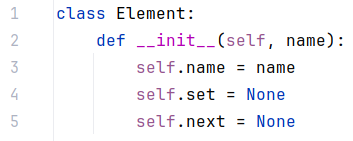
\includegraphics[width=0.5\textwidth]{images/linked_list/ll_element.png}
    \caption{Codice della classe Element per lista concatenata}
    \label{fig:ll_element}
\end{figure}
Un elemento dell'insieme viene rappresentato dalla classe \textit{Element} (Figura \ref{fig:ll_element}) il quale contiene un attributo \textit{name} che funge da rappresentante dell'elemento, un attributo \textit{set} che punta alla lista concatenata rappresentante l'insieme a cui l'elemento appartiene e un attributo \textit{next} che punta al successivo elemento della lista.
Questa classe verrà usata sia nella rappresentazione con euristica dell'unione pesata sia in quella senza euristica.

\subsubsection{Classe LinkedList}
\begin{figure}[h]
    \centering
    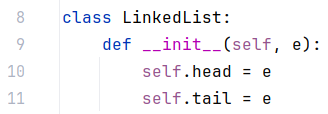
\includegraphics[width=0.5\textwidth]{images/linked_list/ll_class.png}
    \caption{Codice della classe LinkedList}
    \label{fig:ll_class}
\end{figure}
Questa classe rappresenta un insieme (Figura \ref{fig:ll_class}), ha come attributi \textit{head} che punta al rappresentante dell'insieme e \textit{tail} che invece punta all'ultimo elemento della lista.

\subsubsection{Funzione make\_set()}
\begin{figure}[h]
    \centering
    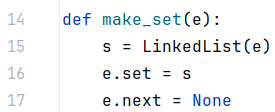
\includegraphics[width=0.5\textwidth]{images/linked_list/ll_make_set.png}
    \caption{Codice della funzione make\_set() per lista concatenata}
    \label{fig:ll_make_set}
\end{figure}
La funzione in Figura \ref{fig:ll_make_set} permette di creare una nuova lista: prende come parametro l'elemento con cui creare l'insieme e ne modifica il puntatore a \textit{set} in modo tale che punti al nuovo insieme creato, inoltre poiché l'insieme contiene un solo elemento imposta il puntatore \textit{next} a None.

\subsubsection{Funzione find()}
\begin{figure}[h]
    \centering
    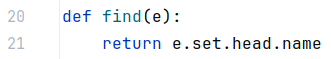
\includegraphics[width=0.5\textwidth]{images/linked_list/ll_find.png}
    \caption{Codice della funzione find() per lista concatenata}
    \label{fig:ll_find}
\end{figure}
Permette di ottenere il \textit{name} del rappresentante dell'insieme a cui appartiene l'elemento passato come parametro (Figura \ref{fig:ll_find}).\\
Questa funzione verrà usata per la rappresentazione tramite lista concatenata sia con che senza euristica dell'unione pesata.

\subsubsection{Funzione union()}
\begin{figure}[h]
    \centering
    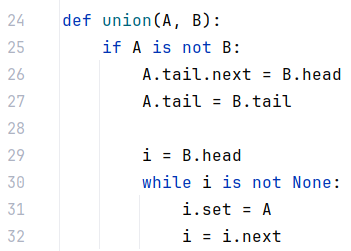
\includegraphics[width=0.5\textwidth]{images/linked_list/ll_union.png}
    \caption{Codice della funzione union()}
    \label{fig:ll_union}
\end{figure}
Nella funzione (Figura \ref{fig:ll_union}) per prima cosa controllo che i due insiemi dati come parametri siano diversi, in tal caso aggiorna il puntatore dell'ultimo elemento dell'insieme \textit{A} in modo che punti al primo elemento dell'insieme \textit{B}, aggiorna il puntatore \textit{tail} dell'insieme \textit{A} facendolo puntare all'ultimo elemento dell'insieme \textit{B}.\
Dopodiché aggiorno tutti i puntatori \textit{set} degli elementi della lista \textit{B} in modo che puntino al nuovo insieme.

\subsubsection{Classe HeuristicsLinkedList}
\begin{figure}[h]
    \centering
    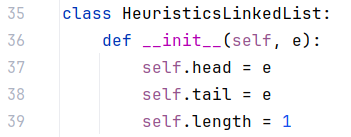
\includegraphics[width=0.5\textwidth]{images/linked_list/llh_class.png}
    \caption{Codice della classe HeuristicsLinkedList}
    \label{fig:llh_class}
\end{figure}
Questa classe (Figura \ref{fig:llh_class}) è per lo più identica alla classe LinkedList, l'unica differenza consiste nell'attributo \textit{length} che registra il numero di elementi all'interno dell'insieme.

\subsubsection{Funzione heuristics\_make\_set()}
\begin{figure}[h]
    \centering
    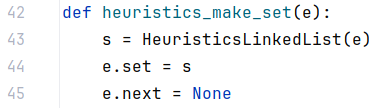
\includegraphics[width=0.5\textwidth]{images/linked_list/llh_make_set.png}
    \caption{Codice della funzione heuristics\_make\_set()}
    \label{fig:llh_make_set}
\end{figure}
Come l'equivalente per la rappresentazione senza euristica, questa funzione (Figura \ref{fig:llh_make_set}) crea un nuovo oggetto di tipo HeuristicsLinkedList e imposta il puntatore \textit{set} dell'elemento passato come parametro alla funzione.

\subsubsection{Funzione heursistics\_union()}
\begin{figure}[h]
    \centering
    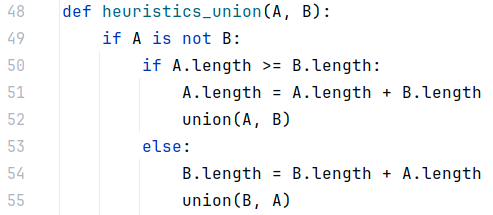
\includegraphics[width=0.5\textwidth]{images/linked_list/llh_union.png}
    \caption{Codice della funzione heuristics\_union()}
    \label{fig:llh_union}
\end{figure}
Come si può osservare dal codice (Figura \ref{fig:llh_union}), la funzione per prima cosa controlla che i due insiemi non siano uguali, dopodiché controlla quale dei due sia quello contenente meno elementi tramite l'attributo \textit{length} e va ad eseguire la funzione \textit{union} definita prima per unire le due liste, andando precedentemente ad aggiornare la lunghezza delle liste.

% ---------- set forest
\subsection{Codice foresta di insiemi disgiunti (set\_forest)}

\subsubsection{Classe Element}
\begin{figure}[h]
    \centering
    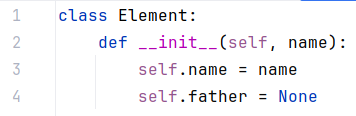
\includegraphics[width=0.5\textwidth]{images/set_forest/sf_element.png}
    \caption{Codice della classe Element per foresta di insiemi disgiunti}
    \label{fig:sf_element}
\end{figure}
Nella rappresentazione tramite foresta di insiemi disgiunti ciascun elemento (Figura \ref{fig:sf_element}) contiene un attributo \textit{name} che svolge il ruolo di rappresentante dell'elemento ed un puntatore \textit{father} che punta al nodo padre dell'elemento.

\subsubsection{Funzione make\_set()}
\begin{figure}[h]
    \centering
    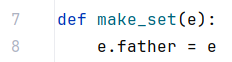
\includegraphics[width=0.4\textwidth]{images/set_forest/sf_make_set.png}
    \caption{Codice della funzione make\_set() per foresta di insiemi disgiunti}
    \label{fig:sf_make_set}
\end{figure}
La funzione (Figura \ref{fig:sf_make_set}) imposta il puntatore \textit{father} a se stesso, in modo da rendere l'elemento passato come parametro radice di un insieme contente solo se stesso.

\subsubsection{Funzione find()}
\begin{figure}[h]
    \centering
    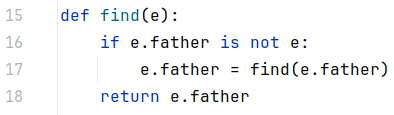
\includegraphics[width=0.5\textwidth]{images/set_forest/sf_find.png}
    \caption{Codice della funzione find() per foreste di insiemi disgiunti}
    \label{fig:sf_find}
\end{figure}
La funzione find() per foresta di insiemi disgiunti (Figura \ref{fig:sf_find}) ritorna un puntatore alla radice dell'elemento, per fare ciò va ad eseguire una chiamata ricorsiva sul padre dell'elemento passato come parametro fino a raggiungere la radice.\\
Nell'eseguire le chiamate ricorsive va anche ad aggiornare il puntatore \textit{father} degli elementi nel cammino di ricerca in modo che abbiano come nodo padre direttamente la radice (in tal modo si implementa la compressione del cammino).

\subsubsection{Funzione union()}
\begin{figure}[h]
    \centering
    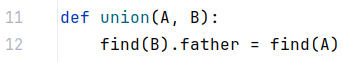
\includegraphics[width=0.5\textwidth]{images/set_forest/sf_union.png}
    \caption{Codice della funzione union() per foresta di insiemi disgiunti}
    \label{fig:sf_union}
\end{figure}
Questa funzione (Figura \ref{fig:sf_union}) va ad unire i due insiemi passati come parametri andando a richiamare la funzione \textit{find()} per trovare la radice dell'insieme \textit{B}, dopodiché aggiusta quest'ultima in modo che il proprio puntatore \textit{father} punti alla radice dell'altro insieme \textit{A}.

% ---------- main
\subsection{Codice di inizializzazione e simulazione dell'esperimento (main)}

\subsubsection{Import}
\begin{figure}[h]
    \centering
    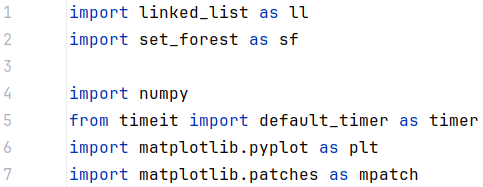
\includegraphics[width=0.5\textwidth]{images/main/import.png}
    \caption{Moduli importati}
    \label{fig:import}
\end{figure}
Nella figura \ref{fig:import} si riportano i moduli importati per l'esecuzione dell'esperimento, più precisamente:
\begin{itemize}
    \item \textbf{linked\_list:} contiene le funzioni e le classi per la rappresentazione tramite lista concatenata, sia con che senza euristica dell'unione pesata.
    \item \textbf{set\_forest:} contiene le classi e le funzioni per la rappresentazione con foresta di insiemi disgiunti e compressione del cammino.
    \item \textbf{numpy:} modulo pyhton usato per la gestione dei vettori e delle matrici usate nell'esperimento, oltre alla generazione randomica degli elementi.
    \item \textbf{timeit:} modulo usato per calcolare i tempi di esecuzione delle varie funzioni, più nello specifico verrà usata la funzione \textit{default\_timer}.
    \item \textbf{matplotlib.pyplot:} modulo usato per creare e salvare su file i vari grafici relativi ai dati raccolti.
    \item \textbf{matplotlib.patches:} modulo python che permette di aggiungere maggiore chiarezza ai grafici generati tramite l'aggiunta di etichette.
\end{itemize}

\subsubsection{Funzione make\_graph}
\begin{figure}[h]
    \centering
    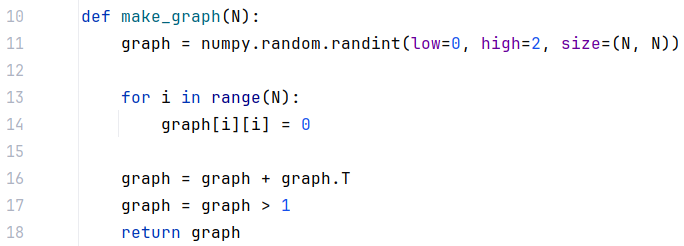
\includegraphics[width=0.6\textwidth]{images/main/make_graph.png}
    \caption{Codice della funzione che genera il grafo}
    \label{fig:make_graph}
\end{figure}
In figura \ref{fig:make_graph} è mostrato il codice che crea una matrice di adiacenza per rappresentare il grafo inserendovi randomicamente gli archi del grafo, successivamente fa alcuni aggiustamenti alla matrice (elimina gli archi sulla diagonale e rende la matrice simmetrica rispetto alla diagonale principale).\\
Essa prende come parametro in ingresso il numero di vertici del grafo.

\subsubsection{Funzioni connect\_componets}
\begin{figure}[h]
    \centering
    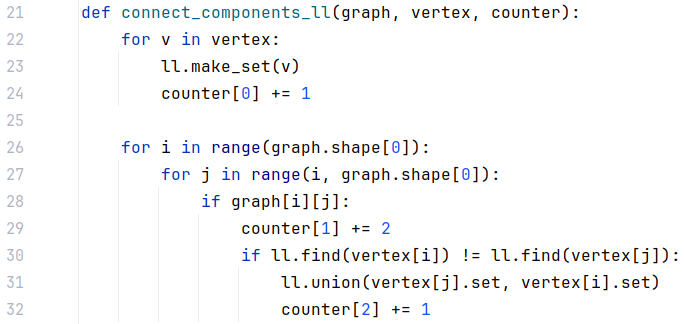
\includegraphics[width=0.6\textwidth]{images/main/connect_components_ll.png}
    \caption{Codice della funzione per il calcolo delle componenti connesse con rappresentazione tramite lista concatenata}
    \label{fig:cc_ll}
\end{figure}
\begin{figure}[h]
    \centering
    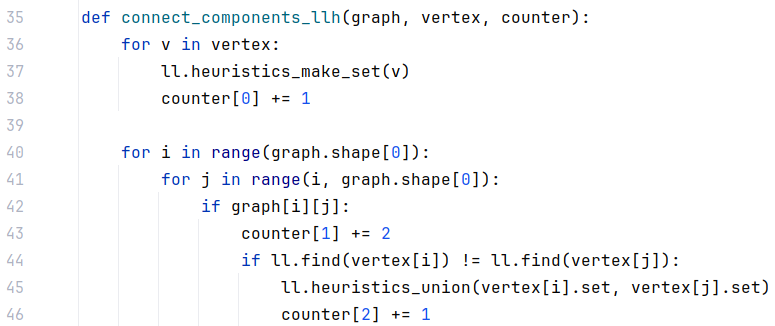
\includegraphics[width=0.6\textwidth]{images/main/connect_components_llh.png}
    \caption{Codice della funzione per il calcolo delle componenti connesse con rappresentazione tramite lista concatenata con euristica dell'unione pesata}
    \label{fig:cc_llh}
\end{figure}
\begin{figure}[h]
    \centering
    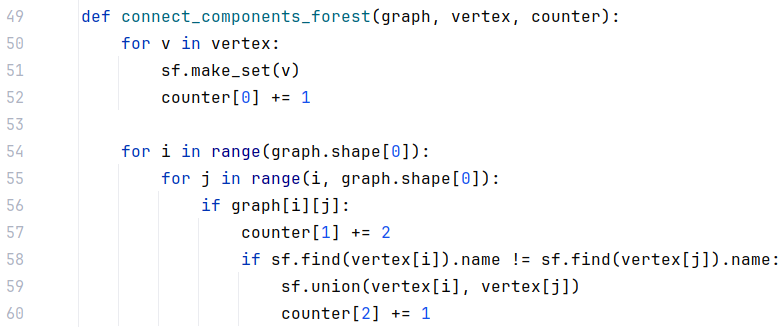
\includegraphics[width=0.6\textwidth]{images/main/connect_components_sf.png}
    \caption{Codice della funzione per il calcolo delle componenti connesse con rappresentazione tramite foresta di insiemi disgiunti}
    \label{fig:cc_sf}
\end{figure}
Nelle figure \ref{fig:cc_ll},\ref{fig:cc_llh} e \ref{fig:cc_sf} è riportato il codice delle funzioni per il calcolo delle componenti connesse con le tre rappresentazioni usate nell'esperimento.
Prendono come parametri \textit{graph}, che è un vettore contenente i vertici del grafo, \textit{vertex} che è la matrice di adiacenza dove sono salvati i vari archi del grafo e \textit{counter}, che è un vettore nel quale viene registrato il numero di operazioni eseguite.\\
Per prima cosa creano per ogni vertice un insieme tramite la corrispettiva funzione \textit{make\_set}, dopodiché esaminano ogni cella della matrice di adiacenza e se l'arco tra i due vertici esiste controllano che i due vertici appartengano a due insiemi diversi tramite \textit{find}: in caso positivo si procedono a fare la \textit{union} dei due insiemi.

\subsubsection{Inizializzazione dell'esperimento}
\begin{figure}[h]
    \centering
    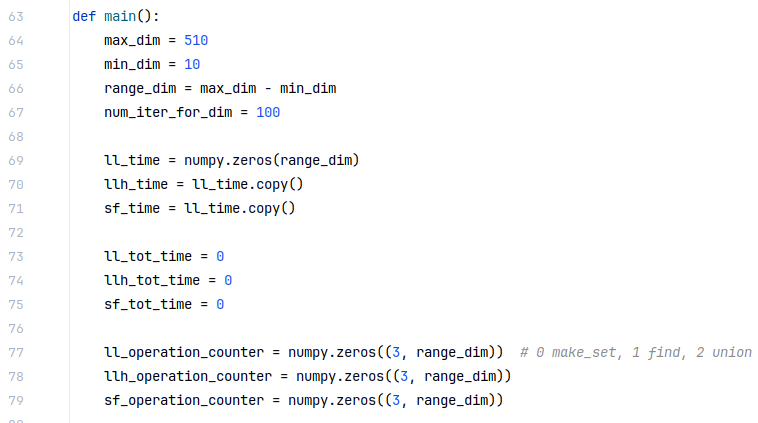
\includegraphics[width=0.6\textwidth]{images/main/main_inizialization.png}
    \caption{Inizializzazione dell'esperimento}
    \label{fig:main_init}
\end{figure}
In questa sezione del modulo dell'esperimento (Figura \ref{fig:main_init}) si inizializzano tutte quelle variabili usate nel corso dell'esperimento, più precisamente:
\begin{itemize}
    \item \textit{range\_dim}: contiene la dimensione dell'insieme dei vertici del grafo.
    \item \textit{num\_iter\_for\_dim}: contiene il numero di volte che si esegue l'esperimento per ogni dimensione dell'insieme dei vertici.
    \item \textit{ll\_time, llh\_time, sf\_time}: verranno usati per registrare i tempi di esecuzione  dell'algoritmo per le componenti connesse delle rispettive metodologie di rappresentazione.
    \item \textit{ll\_tot\_time, llh\_tot\_time, sf\_tot\_time}: permettono di registrare i tempi totali di esecuzione dell'algoritmo per le componenti connesse delle rispettive metodologie.
    \item \textit{ll\_operation\_counter, llh\_operation\_counter, sf\_operation\_counter}: registrano il numero di operazioni per ciascun tipo eseguite durante il calcolo delle componenti connesse.
\end{itemize}

\subsubsection{Cicli di simulazione dell'esperimento}
\begin{figure}[h]
    \centering
    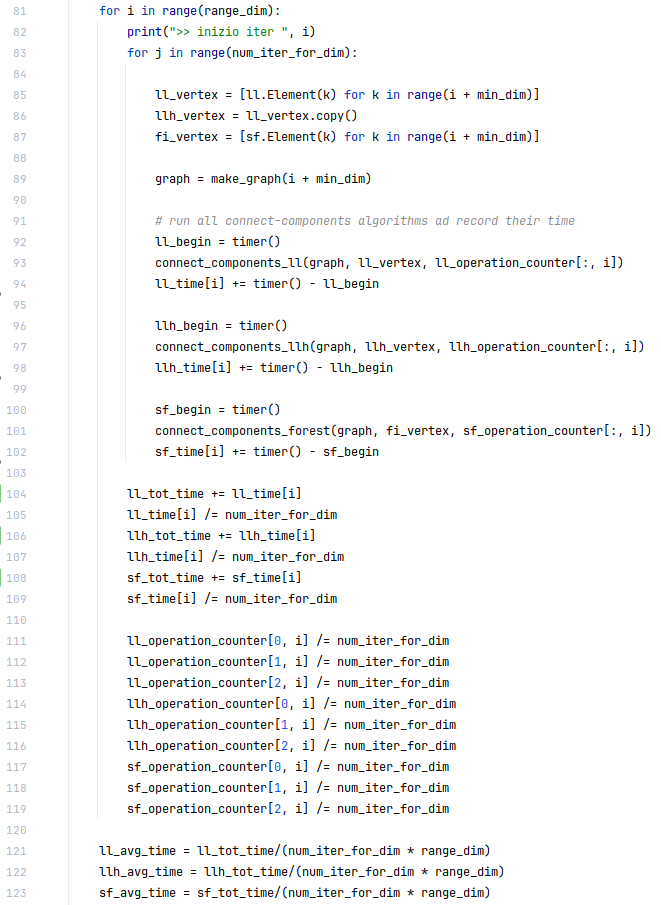
\includegraphics[width=0.7\textwidth]{images/main/main_iterations.png}
    \caption{Cicli esperimento}
    \label{fig:main_cycle}
\end{figure}
Come mostrato in figura \ref{fig:main_cycle}, la simulazione è composta da due cicli: quello più esterno va ad incrementare la dimensione del problema, aumentando il numero di vertici, mentre quello più interno ripete l'esperimento tante volte quante specificate nella variabile \textit{num\_iter\_for\_dim}.\\
All'interno del secondo for vengono generati dei nuovi vettori contenenti i vertici \textit{ll\_vertex, llh\_vertex, sf\_vertex} e un nuovo grafo \textit{graph} tramite la funzione \textit{make\_set} definita sopra.\\
Dopodiché per ogni rappresentazione si esegue il corrispettivo algoritmo per il calcolo delle componenti connesse e si registra il tempo che impiega ad eseguire l'algoritmo con il corrispettivo vettore.\\
Infine, fuori dal ciclo più interno ma sempre dentro a quello più esterno, si vanno ad aggiustare le variabili dividendo per il numero di iterazioni per quella data dimensione.\\
All'esterno dei cicli di simulazione vengono calcolati i tempi medi per ogni dimensione e salvati nelle variabili \textit{ll\_avg\_time, llh\_avg\_time, sf\_avg\_time}.

\subsubsection{Output risultati}
\begin{figure}[h]
    \centering
    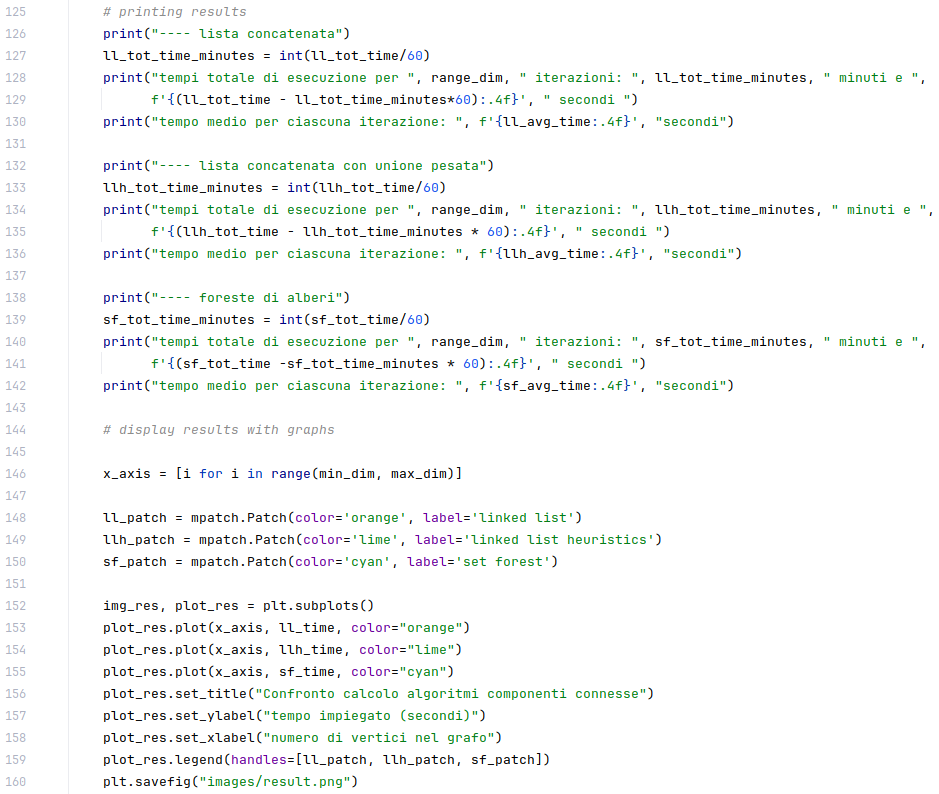
\includegraphics[width=0.7\textwidth]{images/main/main_output.png}
    \caption{Codice per l'output}
    \label{fig:main_output}
\end{figure}
Infine i tempi totali e medi di ciascuna rappresentazioni vengono stampati, inoltre si vanno a creare e salvare su file dei grafici che rappresentino in modo grafico l'andamento dei tempi di esecuzione e del numero di operazioni eseguire all'aumentare del numero di vertici (Figura \ref{fig:main_output}).

% ==============================================================================================
% RISULTATI SPERIMENTALI
% ==============================================================================================
\section{Risultati sperimentali}
Di seguito si mostrano i risultati sui tempi totali e medi ottenuti dall'esperimento:\\
\textit{- lista concatenata\\
tempo totale di esecuzione per  500  iterazioni:  518  minuti e  58.1180  secondi\\
tempo medio per ciascuna iterazione:  0.6228 secondi\\
- lista concatenata con unione pesata\\
tempo totale di esecuzione per  500  iterazioni:  495  minuti e  25.4427  secondi\\
tempo medio per ciascuna iterazione:  0.5945 secondi\\
- foreste di alberi\\
tempo totale di esecuzione per  500  iterazioni:  548  minuti e  4.3195  secondi \\
tempo medio per ciascuna iterazione:  0.6577 secondi\\
}\\
ed i risultati grafici \footnote{si osserva come i grafici del conteggio delle operazioni risultino identici per ogni tipologia di rappresentazione, d'altronde il grafo su cui vengono eseguiti gli algoritmi è lo stesso.\\
I grafici del numero di operazioni di ciascuna tipologia sono riportati per completezza.}, mostrando anche una versione normalizzata per il grafico del numero di operazioni, in modo da mettere meglio in evidenza l'andamento delle operazioni di \textit{find} e \textit{union}:

    \begin{figure}[h]
        \centering
        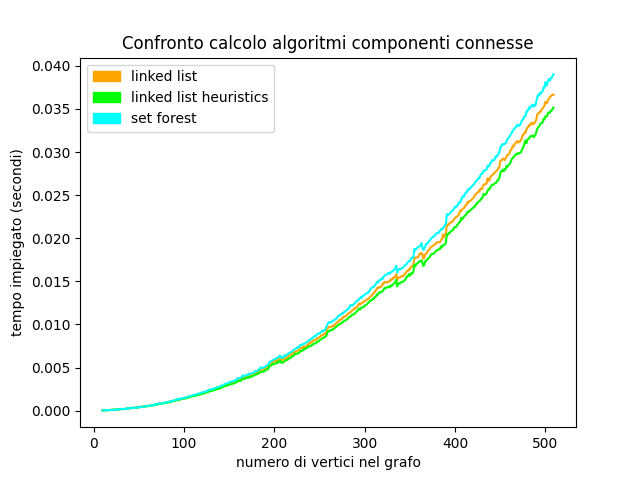
\includegraphics[width=0.7\textwidth]{images/output/result.png}
        \caption{andamento del tempo di esecuzione delle 3 rappresentazioni}
        \label{fig:result}
    \end{figure}

    \begin{figure}[h]
        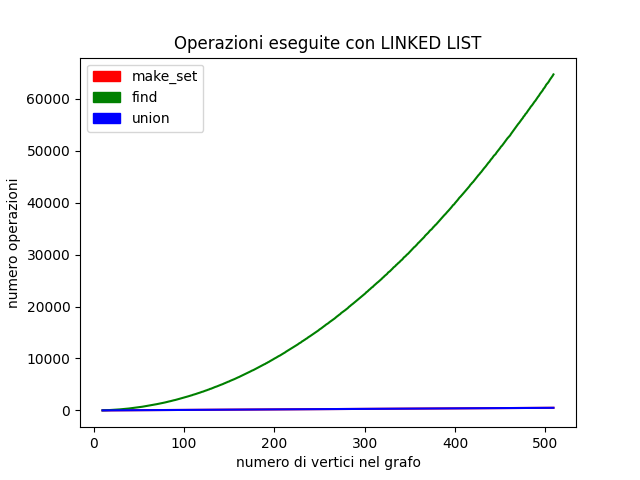
\includegraphics[width=0.7\textwidth]{images/output/count_ll.png}
        \caption{Grafico del numero di operazioni con la rappresentazione tramite lista concatenata}
        \label{fig:count_ll}
    \end{figure}

    \begin{figure}[h]
        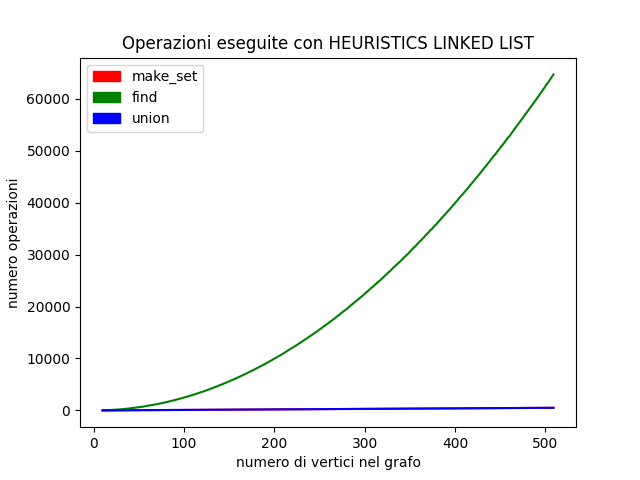
\includegraphics[width=0.7\textwidth]{images/output/count_llh.png}
        \caption{Grafico del numero di operazioni con la rappresentazione tramite lista concatenata ed euristica dell'unione pesata}
        \label{fig:count_llh}
    \end{figure}

    \begin{figure}[h]
        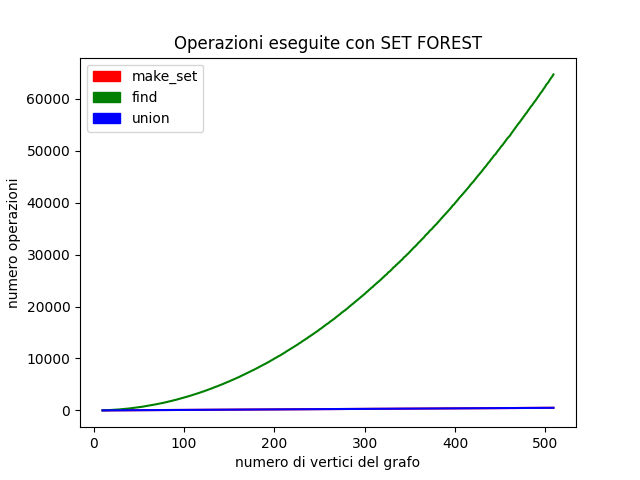
\includegraphics[width=0.7\textwidth]{images/output/count_sf.png}
        \caption{Grafico del numero di operazioni con la rappresentazione tramite foreste di insiemi}
        \label{fig:count_sf}
    \end{figure}

    \begin{figure}[h]
        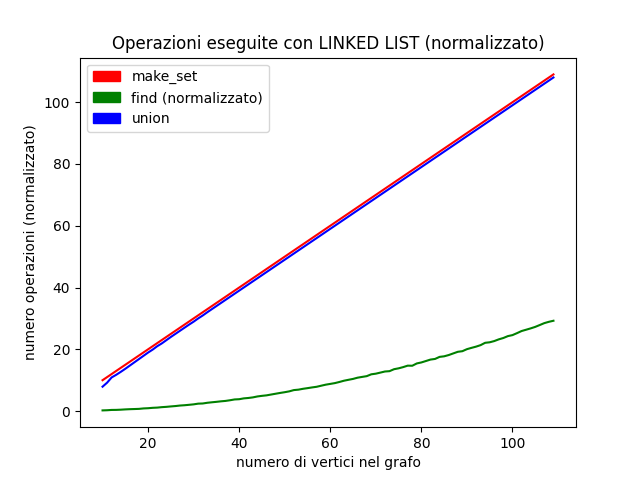
\includegraphics[width=0.7\textwidth]{images/output/count_ll_normalized.png}
        \caption{Grafico del numero di operazioni con la rappresentazione tramite lista concatenata (normalizzato)}
        \label{fig:count_ll_normalized}
    \end{figure}

    \begin{figure}[h]
        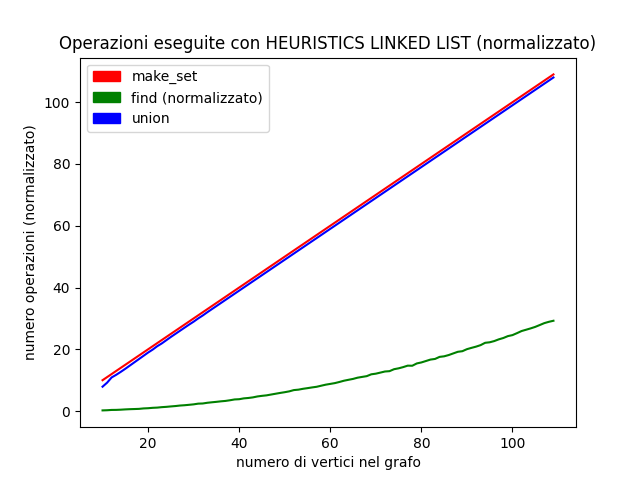
\includegraphics[width=0.7\textwidth]{images/output/count_llh_normalized.png}
        \caption{Grafico del numero di operazioni con la rappresentazione tramite lista concatenata ed euristica dell'unione pesata (normalizzato)}
        \label{fig:count_llh_normalized}
    \end{figure}

    \begin{figure}[h]
        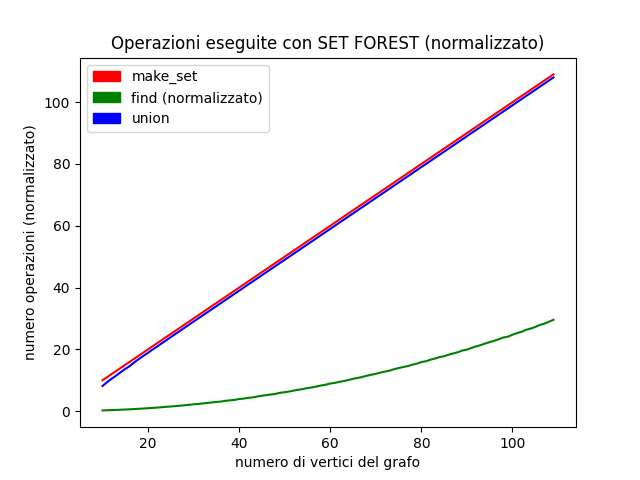
\includegraphics[width=0.7\textwidth]{images/output/count_sf_normalized.png}
        \caption{Grafico del numero di operazioni con la rappresentazione tramite foreste di insiemi (normalizzato)}
        \label{fig:count_sf_normalized}
    \end{figure}


% ==============================================================================================
% DEDUZIONI FINALI
% ==============================================================================================
\section{Deduzioni finali}
Osservando i vari grafici ci si rende conto di come l'andamento sia determinato principalmente dal numero di \textit{find} che vengono eseguiti: infatti risulta che al crescere del numero di vertici il numero di \textit{find} cresca come $\theta(n^2)$, perciò come si può vedere sostituendo il numero di operazioni alle funzioni di costo delle varie rappresentazioni il tempo di esecuzione dell'algoritmo per il calcolo delle componenti connesse cresce più o meno in modo quadratico.\\
La rappresentazione che si dimostra più efficiente è quella tramite \textbf{lista concatenata con euristica dell'unione pesata}, la quale risulta migliore rispetto alla rappresentazione con \textbf{lista concatenata} dato il minor costo dell'operazione di \textit{union}.\\
La rappresentazione mediante \textbf{foresta di insiemi disgiunti} invece risulta quella meno efficiente: a fronte dell'elevato numero di \textit{find} che deve essere eseguito il costo di tale operazione resta troppo alto, perciò la sola euristica di compressione del cammino non risulta sufficiente per avere delle prestazioni migliori rispetto alla rappresentazione mediante lista concatenata.

\printbibliography
%\cite{2010Iaae}
\end{document}